\begin{frame}{$d(K^-, n)"K^0, n"$ vs $K^0 n_{detected}$ invariant mass}
  \tminipageThree{
    \begin{figure}
      Data\\
      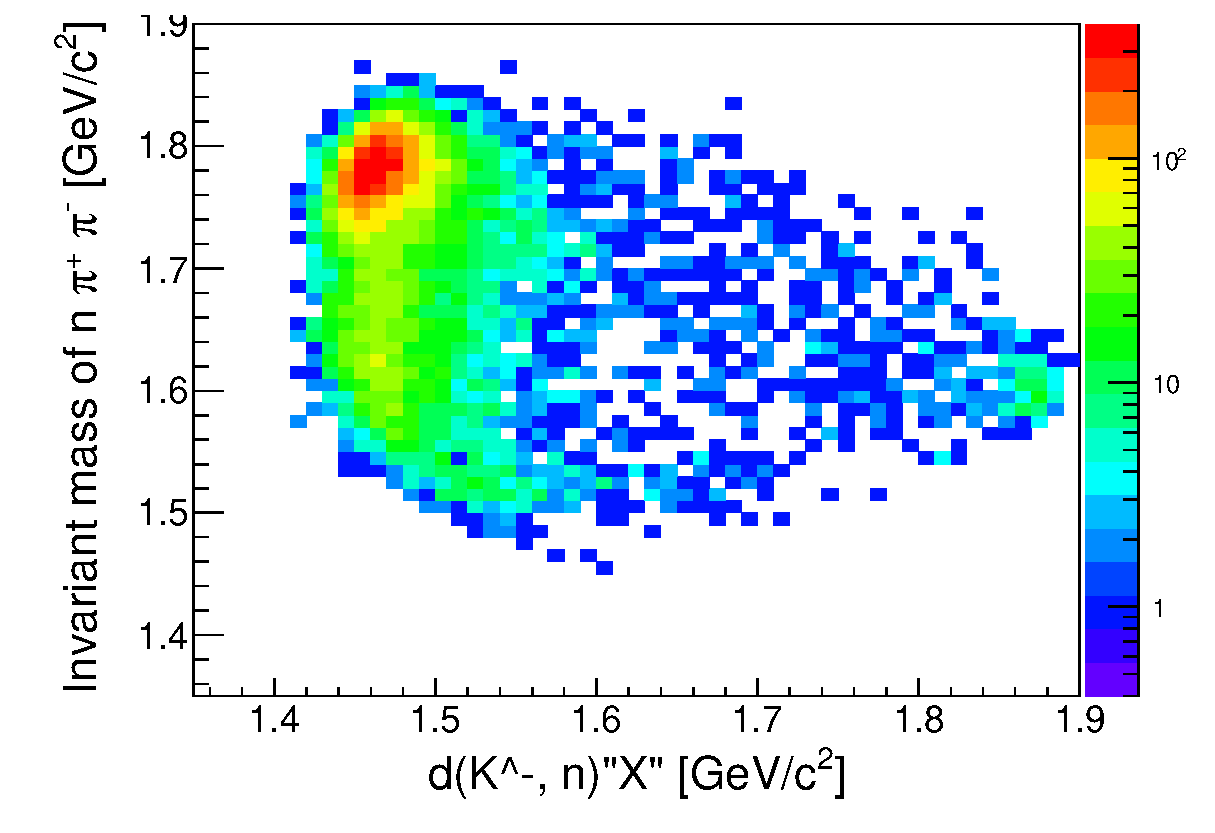
\includegraphics[width=3.5cm]{../pic/Run78/KN_ana/KN_MM_IM_npipi_K0.eps}
    \end{figure}
  }{
    \begin{figure}
      \scriptsize
      $K^-d\rightarrow K^0 n n_{spectator}$ 1step
      \includegraphics[width=3.5cm]{../pic/Run78/KN_ana/KN_MM_IM_npipi_K0_1step}
    \end{figure}    
  }{
    \begin{figure}
      \scriptsize
      $K^-d\rightarrow K^0 n n$ 2step
      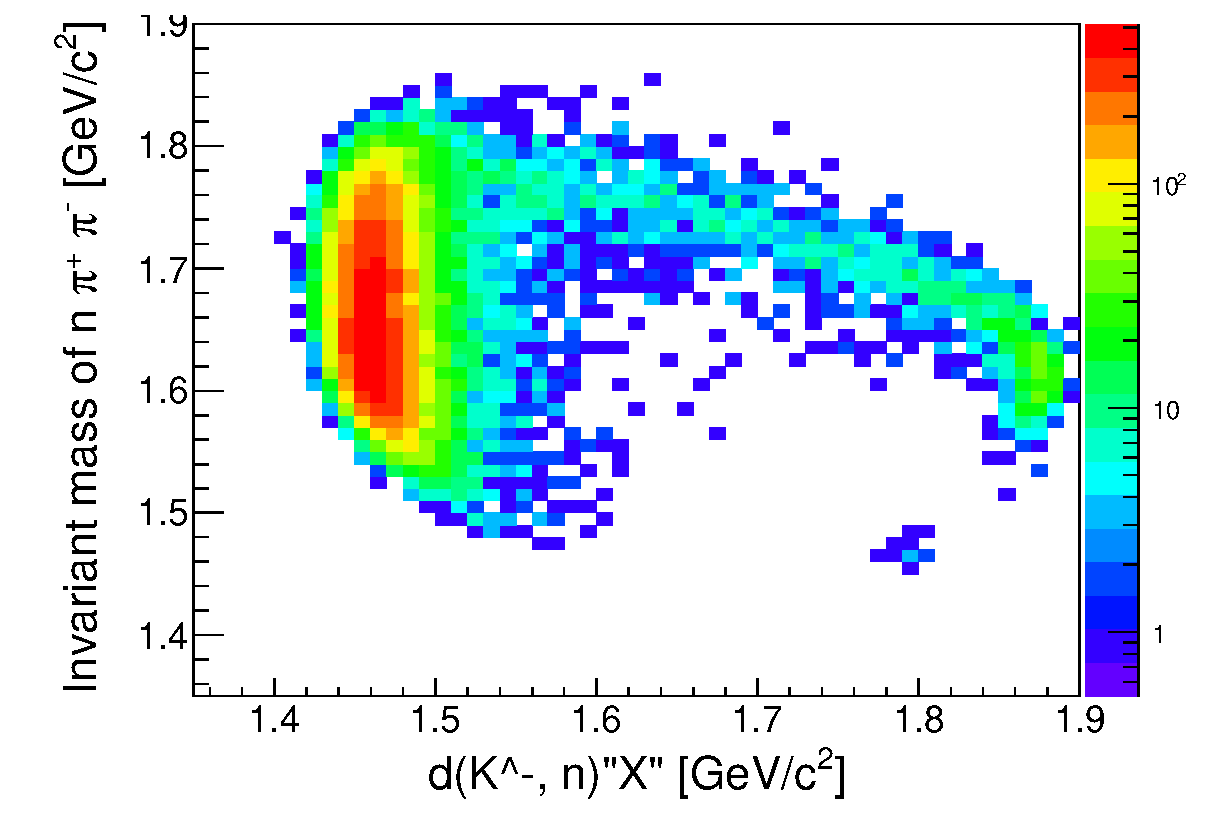
\includegraphics[width=3.5cm]{../pic/Run78/KN_ana/KN_MM_IM_npipi_K0_2step}
    \end{figure}    
  }

  \tminipageThree{
    \centering
    \scriptsize
    2-step : Recolied $\bar{K}$ reacts with residual $N$\\
    \vspace{2mm}
    $K^-d\rightarrow n Y^*$ angular distribution was isotropic
  }{
    \begin{figure}
      \scriptsize
      $K^-d\rightarrow n \Lambda(1520)$ \\
      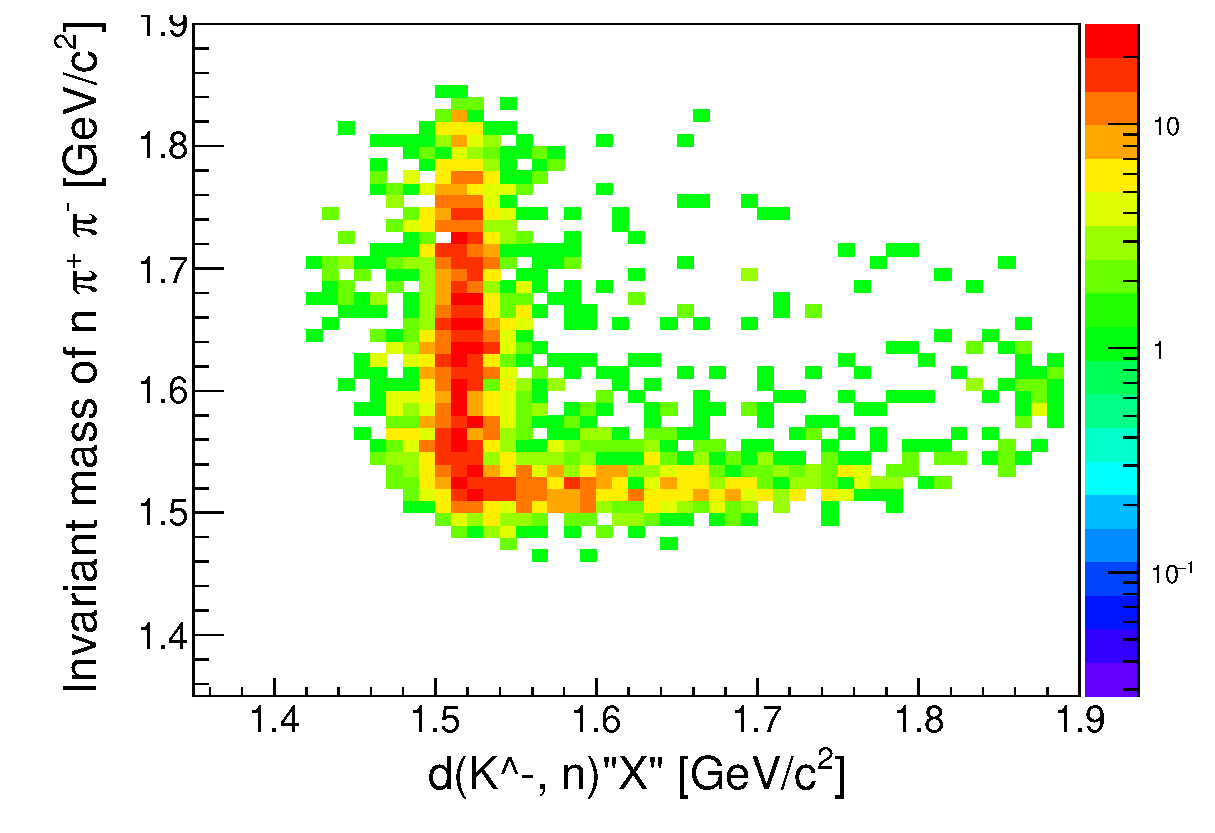
\includegraphics[width=3.5cm]{../pic/Run78/KN_ana/KN_MM_IM_npipi_K0_L1530}
    \end{figure}    
  }{
    \begin{figure}
      \scriptsize
      $K^-d\rightarrow n \Lambda(1600)$ \\
      \includegraphics[width=3.5cm]{../pic/Run78/KN_ana/KN_MM_IM_npipi_K0_L1600}
    \end{figure}    
  }
  \centering
  Widly $Y^*$ contribution distributes high mass of $d(K^-, n)"X"$.\\
  $\rightarrow$ Such reaction can not reproduce data.
\end{frame}
